\begin{frame}
\frametitle{Переупорядочивание}

К сожалению, описанные подходы, как есть, не будут работать...
\begin{itemize}
  \item<2-> компилятору \emph{разрешено} переупорядочивать инструкции:
        \begin{itemize}
          \item компилятор может делать с кодом все, что угодно, пока
                наблюдаемое поведение остается неизменным;
          \item кеширование, удаление "мертвого" кода, спекулятивные записи и
                чтения и многое другое
        \end{itemize}
  \item<3-> процессоры могут использовать оптимизации изменяющие порядок работы
        с памятью:
        \begin{itemize}
          \item store buffer - сохранение данных во временный буффер вместо
                кеша;
          \item invalidate queue - отложенный сброс линии кеша;
        \end{itemize}
\end{itemize}
\end{frame}

\begin{frame}
\frametitle{Оптимизации компилятора}

Компилятор подбирает оптимальный набор инструкций реализующий заданное
наблюдаемое поведение (осторожно C и C++):
\begin{itemize}
  \item обращения к volatile данным (чтение и запись);
  \item операции ввода/вывода (printf, scanf и тд).
\end{itemize}

\onslide<2->{Если компилятору не сообщить, то он не знает:
\begin{itemize}
  \item что переменная может модифицироваться в другом потоке;
  \item что переменную может читать другой поток;
  \item что порядок обращений к переменным важен;
\end{itemize}}
\end{frame}

\begin{frame}
\frametitle{Барьеры компиялтора}

\begin{itemize}
  \item Чтобы сообщить компилятору о "побочных" эффектах работы с памятью
        нужно сделать эту память частью наблюдаемого поведения - использовать
        ключевое слово volatile;
        \begin{itemize}
          \item компилятору запрещено переупорядочивать обращения к volatile
                данным, \emph{если они разделены точкой следования};
          \item компиялтор может переупорядочивать доступ к volatile данным с
                доступом к не volatile данным;
        \end{itemize}
\end{itemize}
\end{frame}

\begin{frame}[fragile]
\frametitle{Барьеры компиялтора}

\begin{columns}[T]
  \begin{column}{.45\linewidth}
    \begin{lstlisting}
struct some_struct {
  int a, b, c;
};

struct some_struct * volatile public;

void foo(void)
{
  struct some_struct *ptr = alloc_some_struct();

  ptr->a = 1;
  ptr->b = 2;
  ptr->c = 3;
  // need something to prevent
  // reordering
  public = ptr;
}
    \end{lstlisting}
  \end{column}
  \begin{column}{.45\linewidth}
    \begin{lstlisting}
void bar(void)
{
  while (!public);
  // and here too
  assert(public->a == 1);
  assert(public->b == 2);
  assert(public->c == 3);
}
    \end{lstlisting}
  \end{column}
\end{columns}
\end{frame}

\begin{frame}[fragile]
\frametitle{Барьеры компиялтора}

Итого: volatile мало чем помогает, что делать? \\
Смотреть в документацию компилятора! Например, gcc предлагает
следующее решение:

\begin{lstlisting}
#define barrier() asm volatile ("" : : : "memory")
\end{lstlisting}
\end{frame}

\begin{frame}[fragile]
\frametitle{Барьеры компиялтора}

\begin{columns}[T]
  \begin{column}{.45\linewidth}
    \begin{lstlisting}
struct some_struct {
  int a, b, c;
};

#define barrier() asm volatile ("" : : : "memory")
struct some_struct *public;

void foo(void)
{
  struct some_struct *ptr = alloc_some_struct();

  ptr->a = 1;
  ptr->b = 2;
  ptr->c = 3;
  barrier();
  public = ptr;
}
    \end{lstlisting}
  \end{column}
  \begin{column}{.45\linewidth}
    \begin{lstlisting}
void bar(void)
{
  while (!public);
  barrier();
  assert(public->a == 1);
  assert(public->b == 2);
  assert(public->c == 3);
}
    \end{lstlisting}
  \end{column}
\end{columns}
\end{frame}

\begin{frame}
\frametitle{Когерентность процессорных кешей}

\begin{figure}
  \only<1>{\centering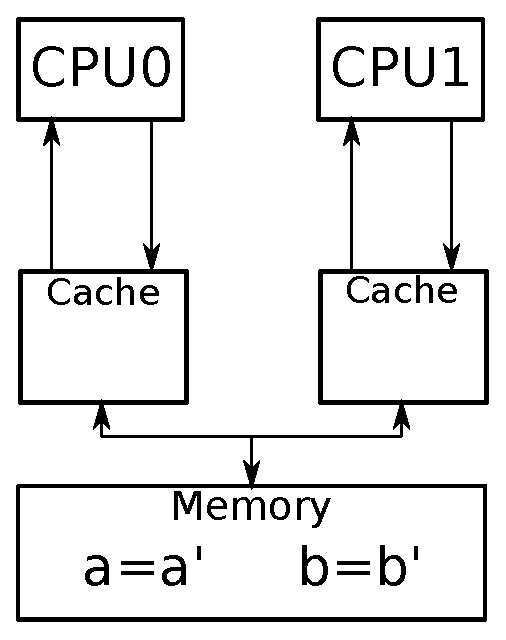
\includegraphics[height=.6\textheight]{cache-coh0}}
  \only<2>{\centering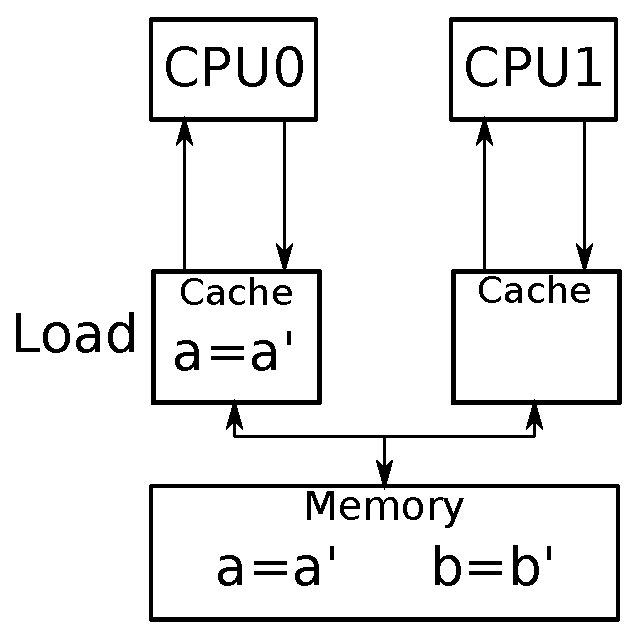
\includegraphics[height=.6\textheight]{cache-coh1}}
  \only<3>{\centering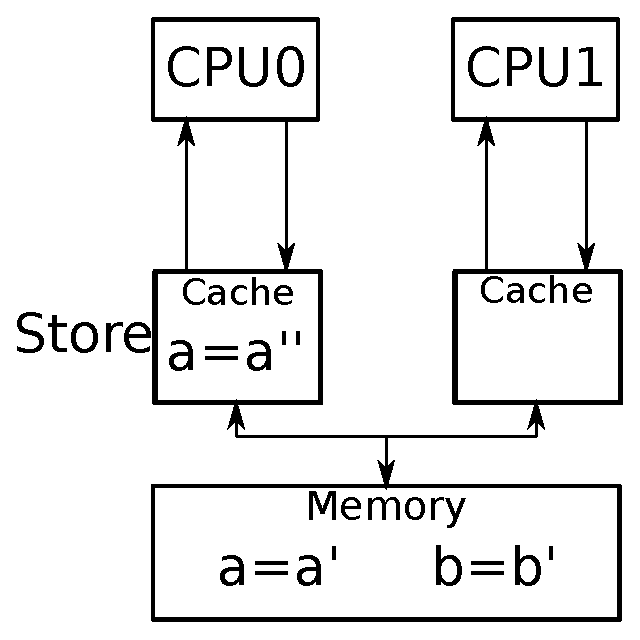
\includegraphics[height=.6\textheight]{cache-coh2}}
  \only<4>{\centering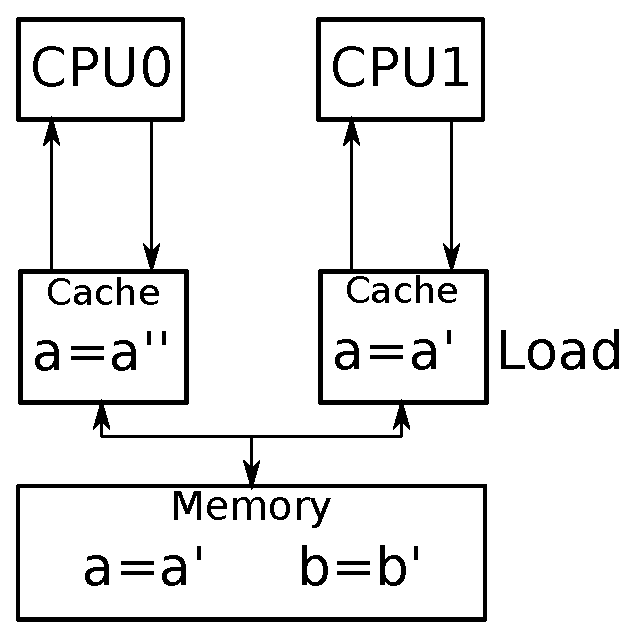
\includegraphics[height=.6\textheight]{cache-coh3}}
  \only<5>{\centering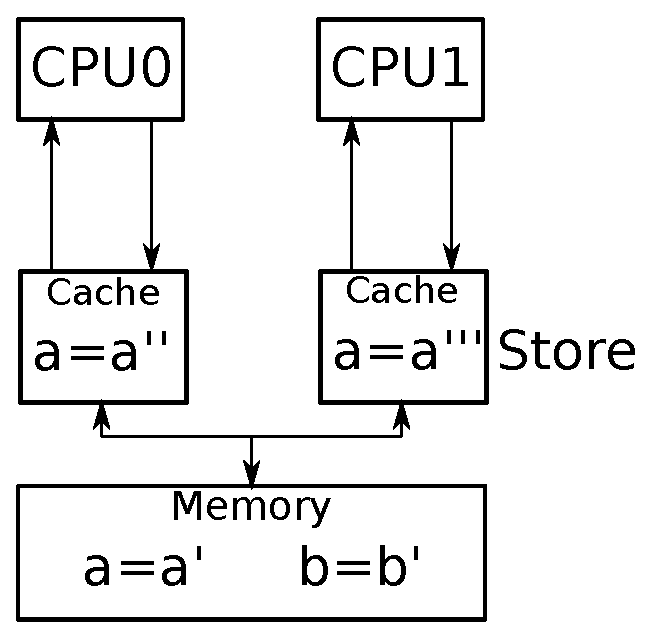
\includegraphics[height=.6\textheight]{cache-coh4}}
  \only<6>{\centering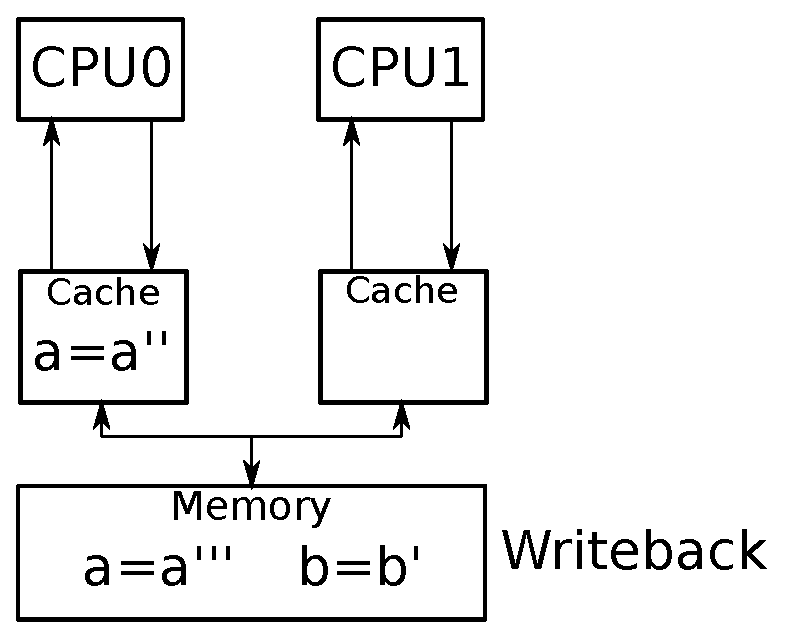
\includegraphics[height=.6\textheight]{cache-coh5}}
  \only<7>{\centering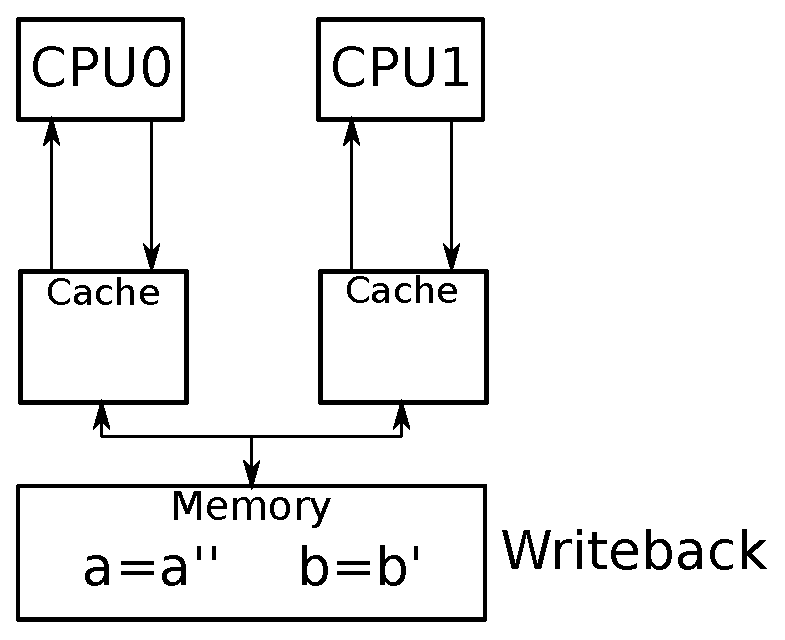
\includegraphics[height=.6\textheight]{cache-coh6}}
  \caption{Cache Incoherency}
\end{figure}
\end{frame}

\begin{frame}
\frametitle{Когерентность процессорных кешей}

Кеши должны находиться в согласованном состоянии (быть когерентными):
\begin{itemize}
  \item процессоры могут обмениваться сообщениями:
        \begin{itemize}
          \item можем считать, что сообщения передаются надежно;
          \item не можем полагаться на порядок доставки и обработки сообщений;
        \end{itemize}
  \item процессоры используют специальный протокол обеспечения когерентности:
        \begin{itemize}
          \item наверно, самый широкоизвестный протокол - MESI (есть сомнения,
                что он используется без модификаций);
        \end{itemize}
\end{itemize}
\end{frame}

\begin{frame}
\frametitle{MESI}
MESI (Modified, Exclusive, Shared, Invalid) предполагает, что каждая линия кеша
находится в одном из четырех состояний:
\begin{itemize}
  \item Modified - кеш линия находится только в кеше данного процессора и она
        была записана (может отличаться от версии в памяти);
  \item Exclusive - кеш линия находится только в кеше данного процессора и она
        совпадает с копией в памяти;
  \item Shared - кеш линия находится в кеше данного процессора и возможно в
        кешах других процессоров, содержимое совпадает с памятью;
  \item Invalid - кеш линия не используется;
\end{itemize}
\end{frame}

\begin{frame}
\frametitle{MESI}
Перед тем как модифицировать данные процессор должен получить данные в
эксклюзивное пользование:
\begin{itemize}
  \item если несколько процессоров держат в кеше данные (Shared), то мы просим
        их сбросить данные;
  \item если другой процессор держит данные в кеше (Modified или Exclusive), то
        мы просим его передать нам данные
        \begin{itemize}
          \item контроллер памяти может увидеть передачу и обновить данные в
                памяти;
          \item или процессор может явно сбросить данные;
        \end{itemize}
  \item если никто не держит данные в кеше, то мы получаем их от контроллера
        памяти;
\end{itemize}
\end{frame}
